\chapter{Implementación}

\section{Modelos implementados}

Un aspecto importante a tener en cuenta sobre la implementación del código es que el desarrollo del código se ha llevado a cabo teniendo en cuenta la calidad del mismo. Además de eso, se han usado características avanzadas de Python como los \textit{type hints} para indicar en el código de que tipo son las variables requeridas por una función y el tipo de variable que devuelve.\newline

Otro aspecto importante que me gustaría recalcar es que todos los modelos han sido testeados usando \textit{Pytest}, lo que me ha permitido encontrar varios bugs antes de ponerme a usarlos.\\

\subsection{Neural Network Classifier}

Este modelo ha sido implementado para poder tener un número variable de capas y de neuronas con el de uasr el optimizador de hiperparámetros. Básicamente, el inicializador tiene como parámetros una lista de número enteros que representa el número de neuronas por cada capa, además de tener otro que representa el número de neuronas en la última capa. Utiliza una \textit{batch normalization} unidimensional y \textit{ReLU} como función de activación. En la última capa hace uso de \textit{Softmax} para calcular la probabilidad de pertenencia a alguna de las clases.\\

\subsection{Convolutional Autoencoder}\label{subsec:cae}

Este modelo fue explicado en la Subsección \ref{subsub:convautoencoder} y tiene los siguientes hiperparámetros:

\begin{itemize}
	\item El número de canales de salida de la primera convolución y el de las siguientes convoluciones se calculan como el número de canales de salida de la anterior multiplicado por dos.
	\item La profundidad del modelo, es decir, cuántas capas convolucionales tiene el \textit{encoder} y el \textit{decoder}.
	\item Tamaño del código del espacio latente.
	\item Número de canales de salida en la primera capa convolucional.
\end{itemize}

Al igual que el \textit{Varitional Autoencoder}, este modelo también hace uso de un \textit{Neural Network Classifier} para la clasificación del código del espacio latente.

\subsection{Convolutional Network Classifier}\label{subsec:convnet}

Este modelo está basado en \textit{LeNet-5} \cite{Lecun98gradient-basedlearning}, con una ligera modificación para poder probar algunas combinaciones en el optimizador de hiperparámetros. Esa modificación es que tiene un número de canales de salida para la convoluciones variable. Este modelo, al igual que los anteriores, usa un modelo de \textit{Neural Network Classifier} a la salida de la última capa de \textit{subsampling}.

\begin{figure}[H]
	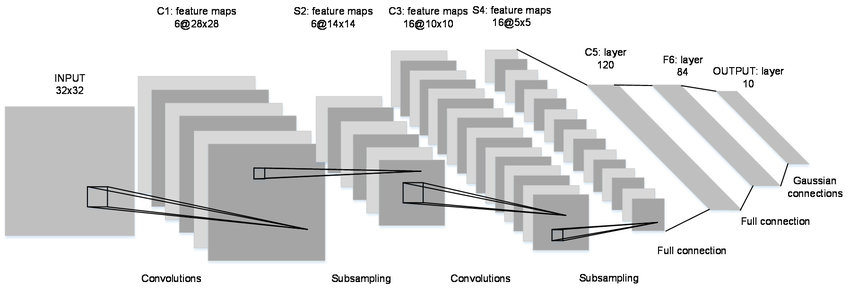
\includegraphics[scale=0.4]{imagenes/05_Implementacion/lenet5.png}
	\centering
	\caption{Estructura de \textit{LeNet-5}. \cite{Lecun98gradient-basedlearning}}
	\label{fig:convnet}
\end{figure}

\subsection{Residual Network Model}\label{subsec:resnetarch}
\label{subsec:resnet}

Para la simplificación del código de este modelo, he creado una clase que contiene las capas convolucionales necesarias para formar un \textit{ResNet block} (se pueden ver ejemplos de estos en la Figura \ref{fig:resnetblocks}). Como se ve en la Figura \ref{fig:resnet}, los \textit{Resnet Blocks} se agrupan en grupos que tienen en común un mismo número de canales en su input. En el primer \textit{ResBlock} de cada grupo, se divide entre dos la altura y la anchura de la imagen y se usa una convolución con tamaño de kernel 1x1 para poder hacer un \textit{downsample} y poder sumar las activaciones de entrada al \textit{ResBlock} con las de salida de la última convolución. Los hiperparámetros de este modelo son:

\begin{itemize}
	\item Número de canales con los que trabaja cada grupo de \textit{ResBlocks}.
	\item Número de \textit{ResBlocks} en cada grupo.
\end{itemize}

Al final de los grupos de \textit{ResBlocks}, uso una capa de \textit{Adaptative Average Pool} para dejar la salida en un vector de tamaño 512x1x1 y usar un \textit{Classifier Neural Network} para clasificar ese \textit{output}.

\begin{figure}[H]
	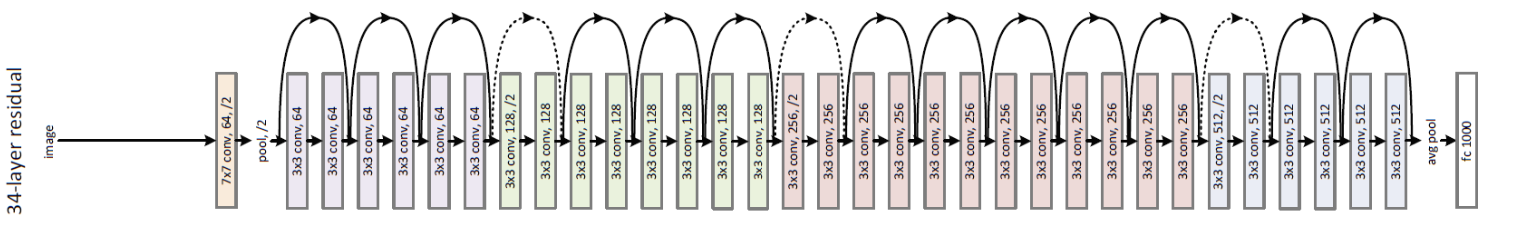
\includegraphics[width=1.\linewidth]{imagenes/05_Implementacion/resnet.png}
	\centering
	\caption{Ejemplo de \textit{ResNet}. \cite{DBLP:journals/corr/HeZRS15}}
	\label{fig:resnet}
\end{figure}

\subsection{Varitional Autoencoder}\label{subsec:vae}

Al igual que el \textit{Neural Network Classifier}, este modelo tiene un número variable de capas y de neuronas por capa. Tiene como parámetro una lista de enteros, que representa el tamaño de las capas del \textit{encoder} si la recorremos de principio a final y la del \textit{decoder} si la recorremos desde el final al principio (el autoencoder es simétrico). A parte, hace uso de una instancia del modelo \textit{Neural Network Classifier} para la clasificación del código latente del autoencoder. Un ejemplo gráfico de este autoencoder puede ser visto en la sección \ref{fig:classiferautoencoder}.\\

\section{Infraestructura Virtual y Metodología de uso}

En las próximas subsecciones se van a detallar las infraestructuras virtuales levantadas para llevar a cabo la realización de este proyecto y el uso que les he dado sin dejar atrás cómo se integran unas con otras.\\

Para este proyecto he diseñado dos infraestructuras diferentes:

\begin{itemize}
    \item \textbf{Infraestructura de test.} Como su propio nombre indica, se encarga de ejecutar los tests y además, de la evaluación del código fuente.
    \item \textbf{Infraestructura de entrenamiento.} Utilizada para entrenar modelos y almacenar los hiperparámetros y las métricas. Para el entrenamiento de los mismos se ha utilizado la GPU de mi portátil personal y las GPUs del clúster \textit{HPMOON}.
\end{itemize}

\subsection{Infraestructura de test}

\begin{figure}[H]
	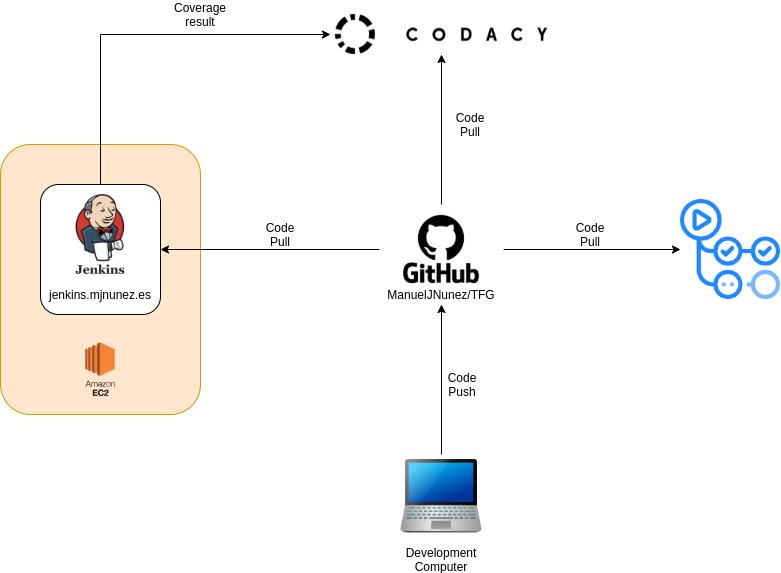
\includegraphics[width=1.\linewidth]{imagenes/05_Implementacion/testinfra.png}
	\centering
	\caption{Esquema de la infraestructura de testing usada en este trabajo.}
\end{figure}

En la imagen de arriba se puede ver la infraestructura virtual para testing que he implementado para llevar a cabo la realización de este proyecto. En esta sección, voy a proceder a describirla por partes:\newline

\begin{itemize}
	\item \textbf{Jenkins.} esta plataforma de CI ha sido alojada en AWS EC2 a través de \textit{Terraform}. El pipeline de Jenkins consta de varios \textit{stages}: el primero instala la dependencias del proyecto, luego se divide en dos caminos paralelos, uno que ejecuta los linters (\textit{Pylint} y \textit{Black}) y otro que ejecuta los tests y envía el resultado de los tests de cobertura a \textit{codacy}.

	\begin{figure}[H]
		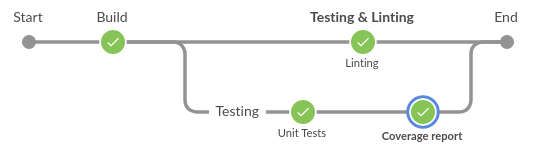
\includegraphics[width=.6\linewidth]{imagenes/05_Implementacion/jenkinspipeline.png}
		\centering
		\captionsetup{justification=centering}
		\caption{Esquema de la infraestructura de testing usada en este trabajo.}
		\label{fig:jenkinspipeline}
\end{figure}

	\item \textbf{Codacy.} esta plataforma se encarga de analizar el código y de guardar los resultados de los tests de cobertura enviados desde Jenkins. Después de analizar el código, muestra los issues del mismo, la complejidad y el porcentaje de código duplicado y le otorga una puntuación desde A hasta F, siendo A la más alta.
	
	\item \textbf{GitHub Actions.} esta plataforma ha sido usada para comprobar la ortografía del README.md, comprobar que no han sido eliminados los ficheros LICENSE, README.md y .gitignore y por último, para probar a ejecutar los tests del código en distintas versiones del intérprete de \textit{Python}, para asegurarme de la versión mínima y máxima en la que se pueden ejecutar los experimentos. 
\end{itemize}

\subsection{Integrando Jenkins con GitHub}

Cuando se usa \textit{Jenkins}, no solo basta con diseñar un \textit{pipeline}. También hay que integrarlo con GitHub para que envíe información sobre el resultado de todos los tests realizados. Esta información se envía en forma de \textit{check}.

\begin{figure}[H]
	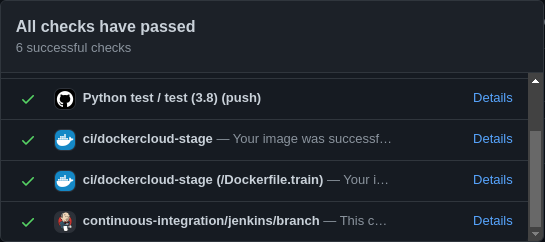
\includegraphics[width=.7\linewidth]{imagenes/05_Implementacion/ghchecks.png}
	\centering
	\caption{Checks en un commit de GitHub.}
	\label{fig:ghchecks}
\end{figure}

Por su parte, \textit{Jenkins} ofrece un plugin muy popular llamado \textit{Open Blue Ocean}, que además de incluir una interfaz web mucho más moderna e intuitiva que la de por defecto, hace uso de otros plugins para integrarse de forma fácil con \textit{GitHub}. Uno de los plugins de los que hace uso se llama \textit{GitHub}, el cual añade un webhook en \textit{Jenkins} para que cada vez que se suban cambios al repositorio, se envíe una notificación para que arranque la \textit{build} automáticamente. Otra \textit{feature} que añade es la de crear \textit{checks} para el commit en el que se está haciendo la \textit{build}.\newline

Para crear el \textit{check}, es necesario autentificar la instancia de \textit{Jenkins} en \textit{GitHub} de alguna manera. Una forma es creando un \textit{Personall Acess Token} en \textit{GitHub}, el problema de esto es que dicha instancia se autentificará como si fuera yo y por tanto usará mi imagen de perfil en los \textit{checks}. ¿Qué ocurre si en la imagen queremos indicar que el \textit{check} ha sido creado por un \textit{Jenkins}? \textit{GitHub} nos ofrece una \textit{feature} para poder integrarlo con plataformas externas, como por ejemplo las de CI/CD. Esto último se llama \textit{GitHub App}, en la cual podemos hacer que reaccione ante los eventos que queramos (\textit{push}, \textit{Pull Request}, nueva \textit{issue}) y notificas a través de una webhook a la plataforma para que reaccione a dichos eventos. Para que eso funcione, debemos de instalarla en el repositorio en el que estemos trabajando. Como se puede ver en la imagen \ref{fig:ghchecks}, uso una imagen del logo de \textit{Jenkins} para indicar el \textit{check} de dicha plataforma.\\

\subsection{Infraestructura de entrenamiento}

\begin{figure}[H]
	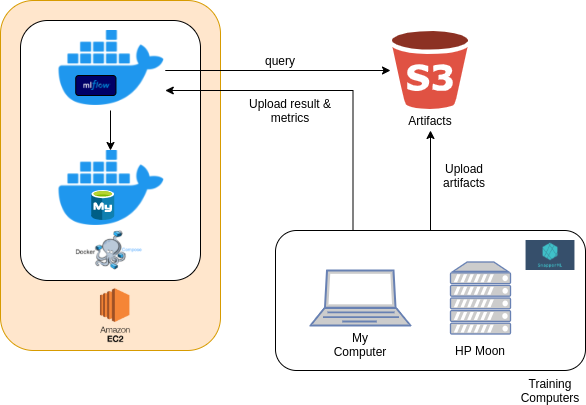
\includegraphics[width=1.\linewidth]{imagenes/05_Implementacion/traininfra.png}
	\centering
	\caption{Esquema de la infraestructura de testing usada en este trabajo.}
\end{figure}

Mi objetivo principal a la hora de realizar la infraestructura de entrenamiento es que la misma se pueda reproducir sólo con unas pocas órdenes, indicadas en el README del repositorio y también en este documento. Esta infraestructura es en realidad muy simple, consta de una instancia de EC2 y un bucket en S3 para guardar artefactos. Por otra parte, el entrenamiento se puede realizar en la máquina directamente teniendo las dependencias instaladas en un entorno virtual gestionado por \textit{poetry} o se puede entrenar usando un contenedor docker si la máquina tiene instalada la herramienta \textit{nvidia-docker2} \cite{nvidiadocker}.\newline

La máquina de EC2 que ejecuta \textit{MLFlow} está aprovisionada con \textit{terraform}, por lo que es perfectamente reproducible. Básicamente, en esta máquina se instala \textit{docker} y \textit{docker-compose} y posteriormente se copian dos ficheros (un \textit{Dockerfile}, un \textit{docker-compose.yml} y un fichero \textit{.env} que contiene la configuración necesaria) que contienen definidos la composición de servicios necesarios para ejecutar \textit{MLFlow}.\newline

En un principio había intentando usar \textit{podman} y \textit{podman-compose}, pero este último no está a la altura de su competidor aún, pues tiene varios problemas y entre ellos el que a mi me acabó afectando fue al no poder crear volúmenes, pues me daba una excepción que yo no podía controlar como usuario, debido a que el código interno de esta herramienta estaba pasando demasiados argumentos a la orden de crear volúmenes, cosa que con \textit{docker-compose} no pasaba. Tal vez \textit{podman} actualizara esa orden, pero no se actualizó en \textit{podman-compose}.\newline

Unos párrafos más atrás, he comentado que para aprovisionar la instancia de \textit{MLFlow}, hace falta un fichero \textit{.env} dentro de \textit{terraform/mlflow/}, dicho fichero debe contener las siguientes claves:

\begin{itemize}
	\item \textbf{MYSQL\_RANDOM\_ROOT\_PASSWORD.} Genera una password aleatoria para el usuario root de la base de datos, por lo que se le debe de asignar cualquier valor (pues será ignorado). También puedes asignarla tú usando la variable MYSQL\_ROOT\_PASSWORD o dejarla vacía usando MYSQL\_ALLOW\_EMPTY\_PASSWORD (inseguro).
	\item \textbf{MYSQL\_USER.} Nombre de usuario no root para acceder a la base de datos. Ejemplo: \textit{mlflow\_user}.
	\item \textbf{MYSQL\_DATABASE.} Nombre de la base de datos que contendrá toda la información sobre los experimentos registrados por mlflow. Ejemplo: \textit{mlflow\_db}.
	\item \textbf{MYSQL\_PASSWORD.} Contraseña para la base de datos que contendrá la información de mlflow. Ejemplo: \textit{mlflow\_pass}.
	\item \textbf{MYSQL\_PORT.} Puerto en el que escuchará el servicio MySQL, en el docker-compose.yml está definido en el 3306, por lo que si se pone uno distinto a ese, se debe actualizar también el otro fichero.
	\item \textbf{MLFLOW\_DBHOST.} Debe contener el valor \textit{mlflow-db}, pues así se llama el servicio de MySQL en el \textit{docker-compose.yml}.
	\item \textbf{MLFLOW\_ARTIFACTS\_URI.} URI en el que se guardarán los artefactos, puede ser local o una dirección de S3 \cite{mlflowtracking}. Ejemplos: \textit{file:///home/mjnunez/mlflow} o \textit{s3://your-bucket/path/to/artifacts}.
	\item \textbf{AWS\_ACCESS\_KEY\_ID.} Si se está usando S3, esto es necesario para la autentificación a la hora de consultar los artefactos.
	\item \textbf{AWS\_SECRET\_ACCESS\_KEY.} Si se está usando S3, esto es necesario para la autentificación, al igual que la clave anterior.
\end{itemize}

Una vez lista la configuración en el fichero, se puede desplegar en una instancia EC2 tan solo escribiendo la orden \textit{terraform apply}.\newline

Para reproducir los experimentos, caben dos posibilidades, o ejecutarlo usando un entorno virtual gestionado por \textit{poetry}, o ejecutarlos dentro de un contenedor que he diseñado para ese propósito (no recomendado, pues el contenedor ocupa 7.01GB). De todos modos, hay que crear otro fichero \textit{.env} en el directorio principal del proyecto con las siguientes claves:

\begin{itemize}
	\item \textbf{POSTGRES\_PASSWORD.} Contraseña para acceder a la base de datos postgres. Ejemplo: \textit{tu-clave123}.
	 \item \textbf{POSTGRES\_USER.} Nombre de usuario para acceder a la base de datos. Ejemplo: \textit{user123}.
	 \item \textbf{POSTGRES\_DB.} Nombre de la base de datos dónde optuna guardará sus datos. Ejemplos: \textit{optuna}.
	 \item \textbf{MLFLOW\_TRACKING\_URI.} dirección URL (o IP) de tu servicio mlflow. Ejemplos: \textit{http://localhost} o \textit{http://mlflow.tu-dominio.com}.
	 \item \textbf{OPTUNA\_STORAGE\_URI.} URI para acceder a la base de datos \textit{posgres}.
	 \item \textbf{AWS\_ACCESS\_KEY\_ID.} Si se está usando S3 en la instancia de \textit{MLflow} para guardar los artefactos, esto es necesario para la autentificación a la hora de subir los artefactos. También se pueden configurar en \textit{$\sim$/.aws/credentials}.
	 \item \textbf{AWS\_SECRET\_ACCESS\_KEY.} Al igual que la variable anterior, sirve para esto es necesario para la autentificación a la hora de subir artefactos. También se pueden configurar en \textit{$\sim$/.aws/credentials}.
\end{itemize}

Una vez configurado todo, podemos arrancar los experimentos con la orden \textit{poetry run inv venvtrain} para ejecutarlo usando los paquetes del entorno virtual de \textit{Python} o usando \textit{poetry run inv dockertrain} para ejecutar los experimentos dentro de un contenedor. A parte de lo anterior, se puede entrenar en otra máquina usando el entorno virtual (en mi caso el HPMoon) a través de SSH usando la siguiente orden:

\begin{lstlisting}[language=bash]
$ poetry run inv sshtrain --destdir=<destination_directory> --host=<server_dir> [--gw=<gw_dir>].
\end{lstlisting}

Sobre la imagen base del contenedor, mi objetivo era que tuviera soporte para usar también GPUs dentro del mismo. Por este mismo motivo, al principio usé \textit{nvidia/cuda:11.3.0-cudnn8-devel-ubuntu20.04}, con la cual terminaba obteniendo una imagen de más de 10GB que no podía construir ni descargar desde un repositorio de contenedores en el HP Moon. Esto era debido a que el tamaño máximo que podía ocupar un contenedor en dicha máquina estaba limitado a 10GB, pero por una petición que le hice al administrador se amplió hasta 20GB. Esto último al final no sirvió, debido a que al final acabé usando una imagen más ligera llamada \textit{nvidia/cuda:11.3.0-cudnn8-runtime-ubuntu20.04}, que también trae las \textit{CUDA math libraries} e incluye \textit{cuDNN}, una biblioteca acelerada por GPU que provee de implementaciones para rutinas estándar como por ejemplo para la \textit{backward propagation} y la \textit{forward propagation}. Esta última es la que usa \textit{PyTorch} a la hora de entrenar modelos por GPU \cite{cudnn}. Como indiqué anteriormente, el tamaño final del contenedor es de 7,01GB.\\

\subsection{Buenas prácticas seguidas a la hora de diseñar los contenedores}\label{subsec:dockerpractices}

A la hora de realizar el proyecto, me he preocupado de seguir las mejores prácticas posibles a la hora de diseñar los \textit{Dockerfiles}. Una de las cosas que más me ha importado ha sido elegir la imagen base más pequeña \cite{dockerbestpracticesdev} (en la subsección anterior ya hablo un poco sobre esto con la imagen de \textit{nvidia/cuda}), por eso en la mayoría de contenedores he usado \textit{python:3.8-slim}. Hay otra imagen más ligera aún que esa llamada \textit{python:3.8-alpine} pero no trae muchas herramientas instaladas y siempre el \textit{workaround} usando estas imágenes es mayor que con otras y suelen acabar ocupando solo un poco menos, por lo que en esta ocasión no compensa tanto ese \textit{workaround}. El uso de esta práctica es necesario para terminar con imágenes finales de poco tamaño y que se puedan ser descargadas en poco tiempo.\newline

Otra práctica interesante que he puesto en práctica también para reducir el volumen de la imagen final, es eliminar la caché del gestor de los gestores de paquetes. Y una que no podemos dejar atrás, reducir el número de capas. Con esto quiero decir que debemos usar el menor número de instrucciones \textit{RUN}, \textit{COPY} y \textit{ADD} que son las que crean las capas. Usarlas frecuentemente implica que el tamaño de la imagen final sea mayor. Por eso, es recomendable encadenar varias órdenes dentro de un mismo \textit{RUN} y así solo se crearía una capa \cite{dockerbestpractices}.\newline

En cuanto a la seguridad del contenedor, siempre es conveniente no usar el usuario \textit{root} que viene por defecto en todos las imágenes de contenedores. Esto es debido a que en caso de un ataque, la superficie sería mayor que usando un usuario que tenga solo acceso a lo justo y necesario, es decir, la aplicación que funcione dentro del contenedor \cite{dockerbestpracticesdev}.\newline

Una buena práctica general de los contenedores es usar cada contenedor para un único propósito. Si desacoplamos aplicaciones entre varios contenedores, el escalado horizontal y el reusar la imagen se hacen más fáciles \cite{dockerbestpractices}.
